\documentclass[10pt]{article}
\usepackage[margin=1in]{geometry}
\usepackage{times}
\usepackage{amsmath,amssymb}
\usepackage{graphicx}
\usepackage{booktabs}
\usepackage{caption}
\usepackage[hidelinks]{hyperref}
\usepackage{xcolor}
\usepackage{titlesec}
\usepackage{enumitem}
\usepackage{authblk}
\captionsetup{font=small,labelfont=bf}
\titleformat{\section}{\large\bfseries}{\thesection}{0.6em}{}
\titleformat{\subsection}{\normalsize\bfseries}{\thesubsection}{0.6em}{}
\setlength{\parskip}{2pt}
\newcommand{\obs}[1]{\textsc{#1}}

\title{\vspace{-2em}\textbf{Selective State-Space Observers for Estimate-Driven\\
Robot Control Under Intermittent Sensing:\\
When Does Open-Loop Accuracy Predict Closed-Loop Performance?}}
\author{Dharini Raghavan}
\affil{\small ECE 6562, Georgia Institute of Technology \\ \texttt{draghavan7}}
\date{\vspace{-1em}\small July 2026}

\begin{document}
\maketitle

\begin{abstract}
\noindent
State estimators for mobile robots are almost always ranked by open-loop accuracy---
position or heading RMSE against ground truth---yet in deployment an estimator is not an end
in itself: its output drives a feedback controller, and what matters is the resulting closed-loop
tracking. We ask whether these two objectives agree. Using a differential-drive robot that
tracks a reference trajectory from noisy odometry and \emph{intermittent} range--bearing landmark
measurements, we compare five observers---dead reckoning, an Extended Kalman Filter (EKF), and
learned recurrent \emph{residual} observers built on GRU and selective (Mamba-style) state-space
cells---inside a closed pure-pursuit loop. Across four physical degradation axes (blackout
duration, measurement noise, landmark density, odometry bias) evaluated over ten seeds each, we
find that open-loop RMSE is a \emph{directionally correct but operationally unreliable} predictor
of closed-loop tracking: rank agreement is high on average (Spearman $\rho=0.89$) but the
correlation of magnitudes is weak (Pearson $r=0.44$) and the \emph{best} observer under open-loop
RMSE is not the best controller in $29\%$ of conditions. The most striking case is our
best-estimating model: a physics-anchored selective-SSM residual on the EKF cuts open-loop
position RMSE by $43\%$ under compound stress yet does \emph{not} improve---and can slightly
worsen---closed-loop cross-track error. We show the physics prior is decisive (dead-reckoning-based
learned observers are open-loop-competitive but closed-loop-unstable) and that removing selectivity
or measurement-mask awareness barely changes open-loop RMSE while causing catastrophic closed-loop
failure. The results extend the objective-mismatch phenomenon of Lambert et al.\ (2020) from
model-based RL to state estimation, and argue for closed-loop-in-the-loop evaluation of learned
filters. All experiments are pure simulation and reproduce from a single command.
\end{abstract}

\section{Introduction}
A robot that localizes well on a bench does not necessarily drive well. In practice a state
estimator is a component in a feedback loop: its pose estimate is consumed by a tracking
controller, whose commands move the robot, which changes what the estimator sees next. The
community nonetheless selects and tunes estimators almost entirely by \emph{open-loop} criteria---
position and heading RMSE against ground truth on logged data---on the implicit assumption that a
more accurate estimate yields better control. This assumption is rarely tested directly, and it is
exactly the kind of \emph{objective mismatch} that Lambert et al.~\cite{lambert} identified for
learned dynamics models in model-based reinforcement learning, where a model with lower one-step
prediction error can produce a worse policy.

We port that question to state estimation under a realistic stressor: \emph{intermittent}
exteroceptive sensing. A differential-drive robot follows a figure-eight reference using
pure-pursuit control~\cite{coulter}. Between landmark sightings it dead-reckons on biased,
noisy wheel odometry; range--bearing measurements to a known map arrive only intermittently and
are periodically blacked out entirely, emulating occlusion, feature dropout, or sensor faults.
Crucially the controller acts on the \emph{estimate}, so estimation error and control error are
coupled through the loop.

Within this testbed we compare a spectrum of observers that share one interface but span the
classical--learned axis: dead reckoning, an EKF~\cite{thrun} with an analytic motion and
measurement model, and \emph{learned residual} observers that add a recurrent correction on top of
a base integrator. For the recurrent core we contrast a GRU against a compact \emph{selective}
diagonal state-space cell in the style of S4/Mamba~\cite{s4,mamba}, whose input-dependent gating
lets it modulate how much it trusts a measurement---a natural inductive bias when measurements
appear and vanish. We evaluate every observer both open-loop (replay RMSE on identical inputs) and
closed-loop (driving the controller), under four degradation axes.

\paragraph{Contributions.}
\begin{enumerate}[leftmargin=1.4em,itemsep=1pt,topsep=1pt]
\item A controlled, fully-reproducible simulation study that measures, rather than assumes, the
relationship between open-loop estimation accuracy and closed-loop tracking for a family of
classical and learned observers under intermittent sensing.
\item Direct evidence of \emph{objective mismatch in state estimation}: open-loop RMSE ranks
observers correctly on average ($\rho=0.89$) but its magnitude correlation is weak ($r=0.44$) and
it selects the wrong observer in $29\%$ of conditions; the best-estimating learned observer does
not minimize closed-loop error.
\item An ablation isolating \emph{why}: a physics prior (EKF anchor) and measurement-mask-aware
selective gating are each necessary for closed-loop stability, even though neither is required for
competitive open-loop RMSE.
\end{enumerate}

\section{Related Work}
\textbf{Classical estimation and tracking.} The EKF and its relatives are the standard tools for
nonlinear robot localization~\cite{thrun,siegwart}. On the control side, pure
pursuit~\cite{coulter} and the Lyapunov-based Kanayama controller~\cite{kanayama} are canonical
trajectory-tracking laws for nonholonomic vehicles; both consume a pose and are agnostic to how it
was produced, which is precisely what lets us swap observers underneath a fixed controller.

\textbf{Learned and hybrid filters.} A large body of work replaces or augments the filter with
neural components: deep variational Bayes filters~\cite{dvbf}, recurrent Kalman
networks~\cite{rkn}, differentiable particle filters~\cite{dpf}, latent-ODE
models for irregular sampling~\cite{latentode}, and KalmanNet~\cite{kalmannet}, which learns the
Kalman gain while retaining the model-based recursion. Our learned observers follow this hybrid
spirit---a residual correction on an analytic base---but differ in \emph{how we evaluate them}:
inside the control loop rather than on estimation error alone.

\textbf{State-space sequence models.} Structured state-space models (S4)~\cite{s4} and the
selective SSM of Mamba~\cite{mamba} make linear recurrences expressive and input-adaptive. Their
selectivity---input-dependent state-transition and input gates---maps naturally onto intermittent
sensing, where the estimator should modulate its reliance on measurements as they appear and
disappear. We use a compact diagonal selective cell as one of our recurrent cores.

\textbf{Objective mismatch.} Lambert et al.~\cite{lambert} showed in model-based RL that lower
model prediction error need not yield better control, decoupling the surrogate training objective
from task performance. We argue the same decoupling arises for observers---between open-loop RMSE
and closed-loop tracking---and measure it directly.

\section{Problem Formulation}
\textbf{Robot and reference.} The robot state is $s=(x,y,\theta)$ with unicycle kinematics
$\dot{x}=v\cos\theta,\ \dot{y}=v\sin\theta,\ \dot\theta=\omega$, integrated at $\mathrm{d}t=0.1$\,s.
The reference is a lemniscate (figure-eight) with a nominal forward speed; the controller must both
translate and turn, exercising heading estimation.

\textbf{Proprioception.} Odometry is corrupted by a multiplicative wheel-slip factor on linear
velocity, an additive gyro bias on angular velocity, and Gaussian noise:
$\tilde v = \kappa\, v + \varepsilon_v,\ \tilde\omega = \omega + b_g + \varepsilon_\omega$.
Slip $\kappa$ and bias $b_g$ create a \emph{systematic} model error---the regime where a fixed
analytic filter is expected to struggle and a learned residual might help.

\textbf{Exteroception and blackouts.} The robot senses range and bearing to a known map of eight
landmarks, but only those within a finite sensor range and within a randomly-drawn active subset
are observed at each step. A periodic schedule blacks out \emph{all} measurements for a fixed
duration, so the estimator must coast on odometry through gaps. A binary mask records which
measurements are present at each step; mask-aware observers see it as an input feature.

\textbf{Closed loop and metrics.} At each step the controller reads the \emph{estimated} pose,
emits $(v,\omega)$ under actuator limits, the true state advances, and new (masked) measurements
are drawn. We report open-loop position/heading RMSE (estimate vs.\ ground truth on identical
replayed inputs) and closed-loop cross-track RMSE, control effort ($\overline{\omega^2}$), recovery
time after blackouts, and a divergence rate (fraction of steps beyond a $1$\,m tube).

\section{Observers}
All observers share the interface \texttt{reset($s_0$)} and \texttt{step($u_{\text{odo}},z,\text{mask},k)\!\to\!\hat s$}.

\textbf{Baselines.} \obs{Dead reckoning} integrates odometry only. The \obs{EKF}~\cite{thrun} uses
the analytic unicycle motion model with assumed process noise and performs range--bearing updates
for whichever landmarks are unmasked, giving a strong model-based reference.

\textbf{Learned residual observers.} Each learned observer wraps a base integrator (dead reckoning
or the EKF) and adds a recurrent correction: $\hat s_k = \text{anchor}_k \oplus r_k$, where a
recurrent cell maps a per-step feature vector---odometry increments, per-landmark
$(\text{range},\sin b,\cos b,\text{mask})$ tuples, an anchor-pose encoding, and (for EKF-anchored
variants) the EKF covariance diagonal---to a small pose residual $r_k$. The readout is initialized
near zero so each learned observer \emph{starts} equal to its analytic prior and only learns to
correct it. We train by backpropagation through time on domain-randomized expert rollouts, with a
position-MSE plus heading cosine loss.

\textbf{Recurrent cores.} We compare a \textbf{GRU} against a \textbf{selective diagonal SSM}: a
linear recurrence $h_k=\bar A_k h_{k-1}+\bar B_k u_k$, $r_k=C_k h_k$ with a stable parameterization
$A=-\mathrm{softplus}(\cdot)$ and \emph{input-dependent} step size, input and output gates
($\Delta_k,B_k,C_k$ functions of the feature), following the selective-SSM idea~\cite{mamba}. A
non-selective variant fixes these gates as constants. Selectivity lets the observer, in principle,
down-weight state propagation during blackouts and re-engage measurements on return.

This yields our zoo: \obs{DR}, \obs{EKF}, \obs{GRU-DR}, \obs{SSM-DR} (selective), \obs{SSM-EKF}
(selective, covariance-aware) and \obs{GRU-EKF}, plus non-selective and mask-free ablations.

\section{Experimental Setup}
The world is fully synthetic---no external datasets---which makes the study exactly reproducible
and matches standard practice for learned-filter benchmarks. Learned observers are trained on
$200$ domain-randomized trajectories ($200$ steps) with all four degradation axes randomized, using
Adam with gradient clipping and early stopping on a held-out set; a single training seed is used per
model. Evaluation uses \emph{fresh} seeds and randomized active-landmark subsets. The nominal
evaluation applies mild mismatch; each degradation axis is then swept over six levels while holding
the others at nominal, with ten evaluation seeds per level. For every condition we compute both the
closed-loop metrics and, on separate expert-replayed inputs shared across observers, the open-loop
RMSE---so open- and closed-loop numbers are directly comparable. Training a full model takes
$\sim$1--3\,min on a single CPU core; the entire sweep runs in a few minutes.

\begin{figure}[t]
\centering
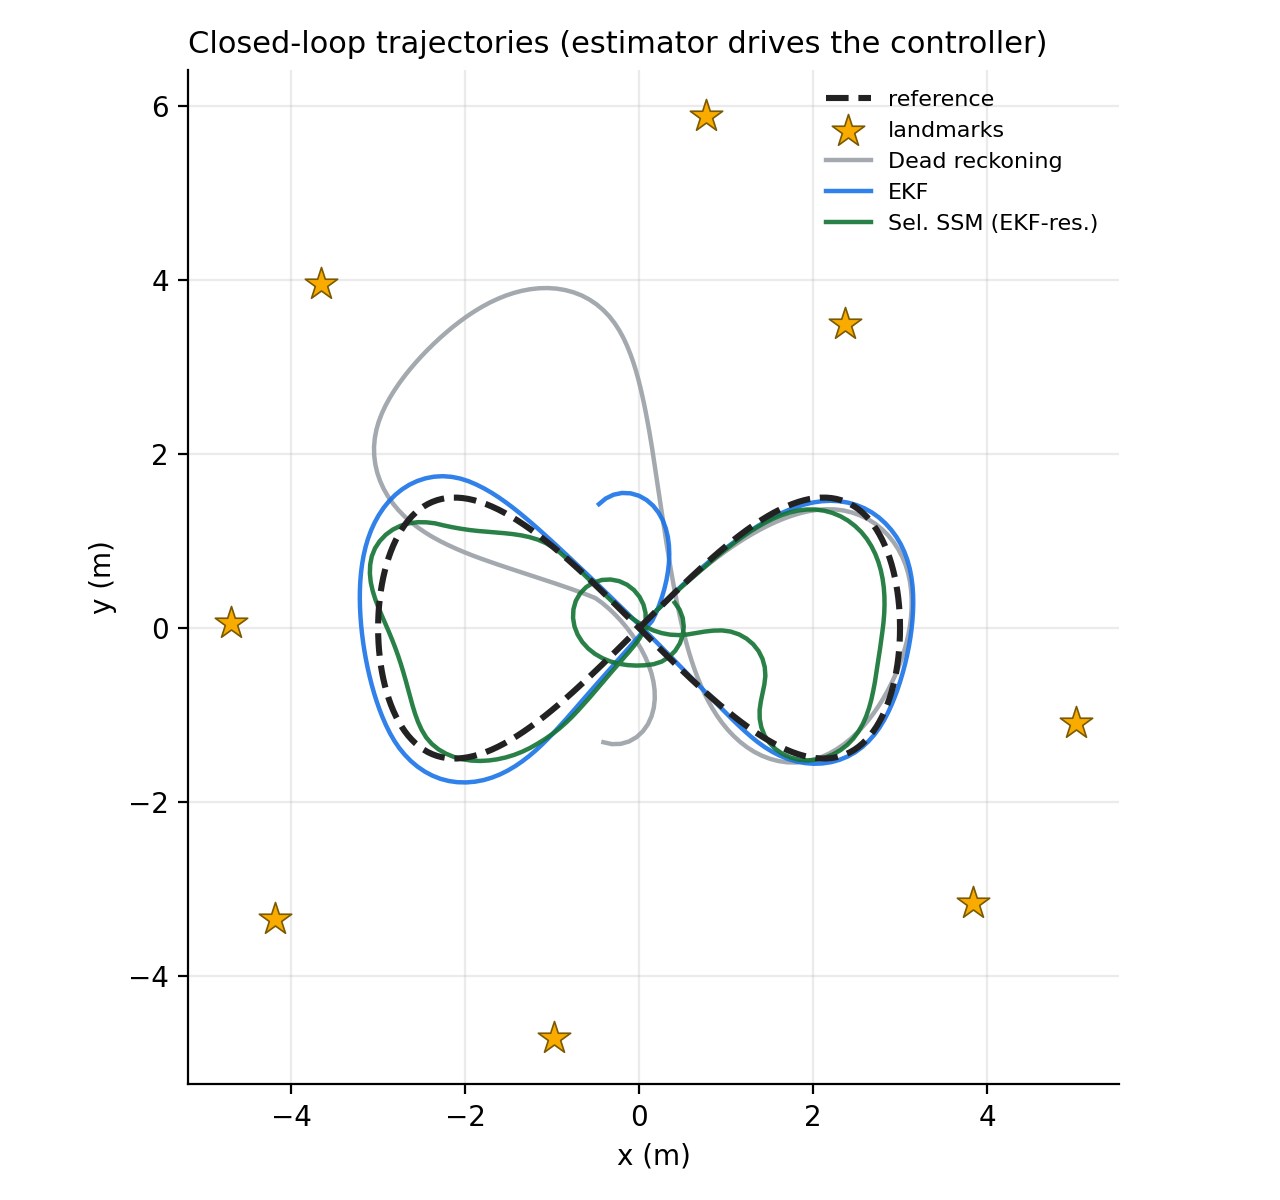
\includegraphics[width=0.62\linewidth]{fig_trajectory.png}
\caption{Closed-loop trajectories under nominal mismatch. Dead reckoning drifts off the reference
between landmark sightings; the EKF and the selective-SSM EKF-residual observer both track the
figure-eight closely. The controller acts on each observer's estimate, so drift becomes tracking
error.}
\label{fig:traj}
\end{figure}

\section{Results}
\subsection{Nominal operating point}
Table~\ref{tab:nominal} reports the nominal comparison. The EKF is already an excellent baseline
(closed-loop cross-track $0.21$\,m, zero divergence). The EKF-residual learned observers match or
slightly beat it (\obs{GRU-EKF} $0.16$\,m, \obs{SSM-EKF} $0.20$\,m) and achieve the best open-loop
RMSE. The dead-reckoning-residual learned observers tell the first cautionary tale: despite
\emph{excellent} open-loop position RMSE ($0.28$--$0.33$\,m, $4$--$5\times$ better than raw dead
reckoning), their closed-loop cross-track error is $0.69$--$0.91$\,m with large variance and
nonzero divergence---far worse than the EKF they never see. Good estimates on replayed data did not
survive contact with the loop.

\begin{table}[t]
\centering\small
\caption{Nominal evaluation (mild mismatch), mean over 10 seeds; $\pm$ is the $95\%$ CI half-width.
Cross-track (CT) and position are closed-loop; OL-Pos is open-loop replay position RMSE. Lower is
better throughout. Learned dead-reckoning-residual observers estimate well open-loop yet control
poorly.}
\label{tab:nominal}
\begin{tabular}{lccccc}
\toprule
Observer & CT RMSE (m) & Pos RMSE (m) & Effort & OL-Pos (m) & Div. \\
\midrule
Dead reckoning        & $1.045\pm.03$ & $1.834\pm.04$ & $0.45$ & $1.503\pm.20$ & $0.26$ \\
EKF                   & $0.212\pm.02$ & $0.146\pm.01$ & $0.68$ & $0.140\pm.01$ & $0.00$ \\
GRU (DR-residual)     & $0.694\pm.35$ & $1.033\pm.37$ & $0.91$ & $0.281\pm.03$ & $0.14$ \\
Sel.\ SSM (DR-res.)   & $0.909\pm.50$ & $1.399\pm.81$ & $1.12$ & $0.325\pm.04$ & $0.20$ \\
Sel.\ SSM (EKF-res.)  & $0.199\pm.03$ & $0.191\pm.04$ & $1.05$ & $0.121\pm.02$ & $0.00$ \\
GRU (EKF-residual)    & $\mathbf{0.163\pm.02}$ & $0.109\pm.01$ & $0.95$ & $\mathbf{0.094\pm.01}$ & $0.00$ \\
\midrule
\multicolumn{6}{l}{\emph{ablations}}\\
SSM, no selectivity   & $3.255\pm1.04$ & $4.313\pm1.15$ & $0.90$ & $0.588\pm.06$ & $0.58$ \\
SSM, no mask          & $2.292\pm1.58$ & $3.910\pm2.83$ & $1.09$ & $0.301\pm.03$ & $0.32$ \\
\bottomrule
\end{tabular}
\end{table}

\subsection{Degradation sweeps}
Figure~\ref{fig:sweeps} sweeps each axis. Two patterns recur. First, the ordering among the
\emph{strong} observers (EKF and the two EKF-residual hybrids) is regime-dependent: the learned
residual helps most where measurements are \emph{frequent but mis-modeled}---at the highest range
noise ($\sigma_r=0.5$) the selective SSM-EKF cuts cross-track error by $26\%$ vs.\ the EKF
($0.31$ vs.\ $0.42$\,m), and at the largest gyro bias ($0.25$) by $29\%$ ($0.31$ vs.\ $0.44$\,m).
Second, the residual does \emph{not} help where information is simply absent: under the longest
blackouts the EKF edges out the hybrids, and with only two landmarks the two are tied---consistent
with a learned correction having nothing to correct when measurements vanish.

\begin{figure}[t]
\centering
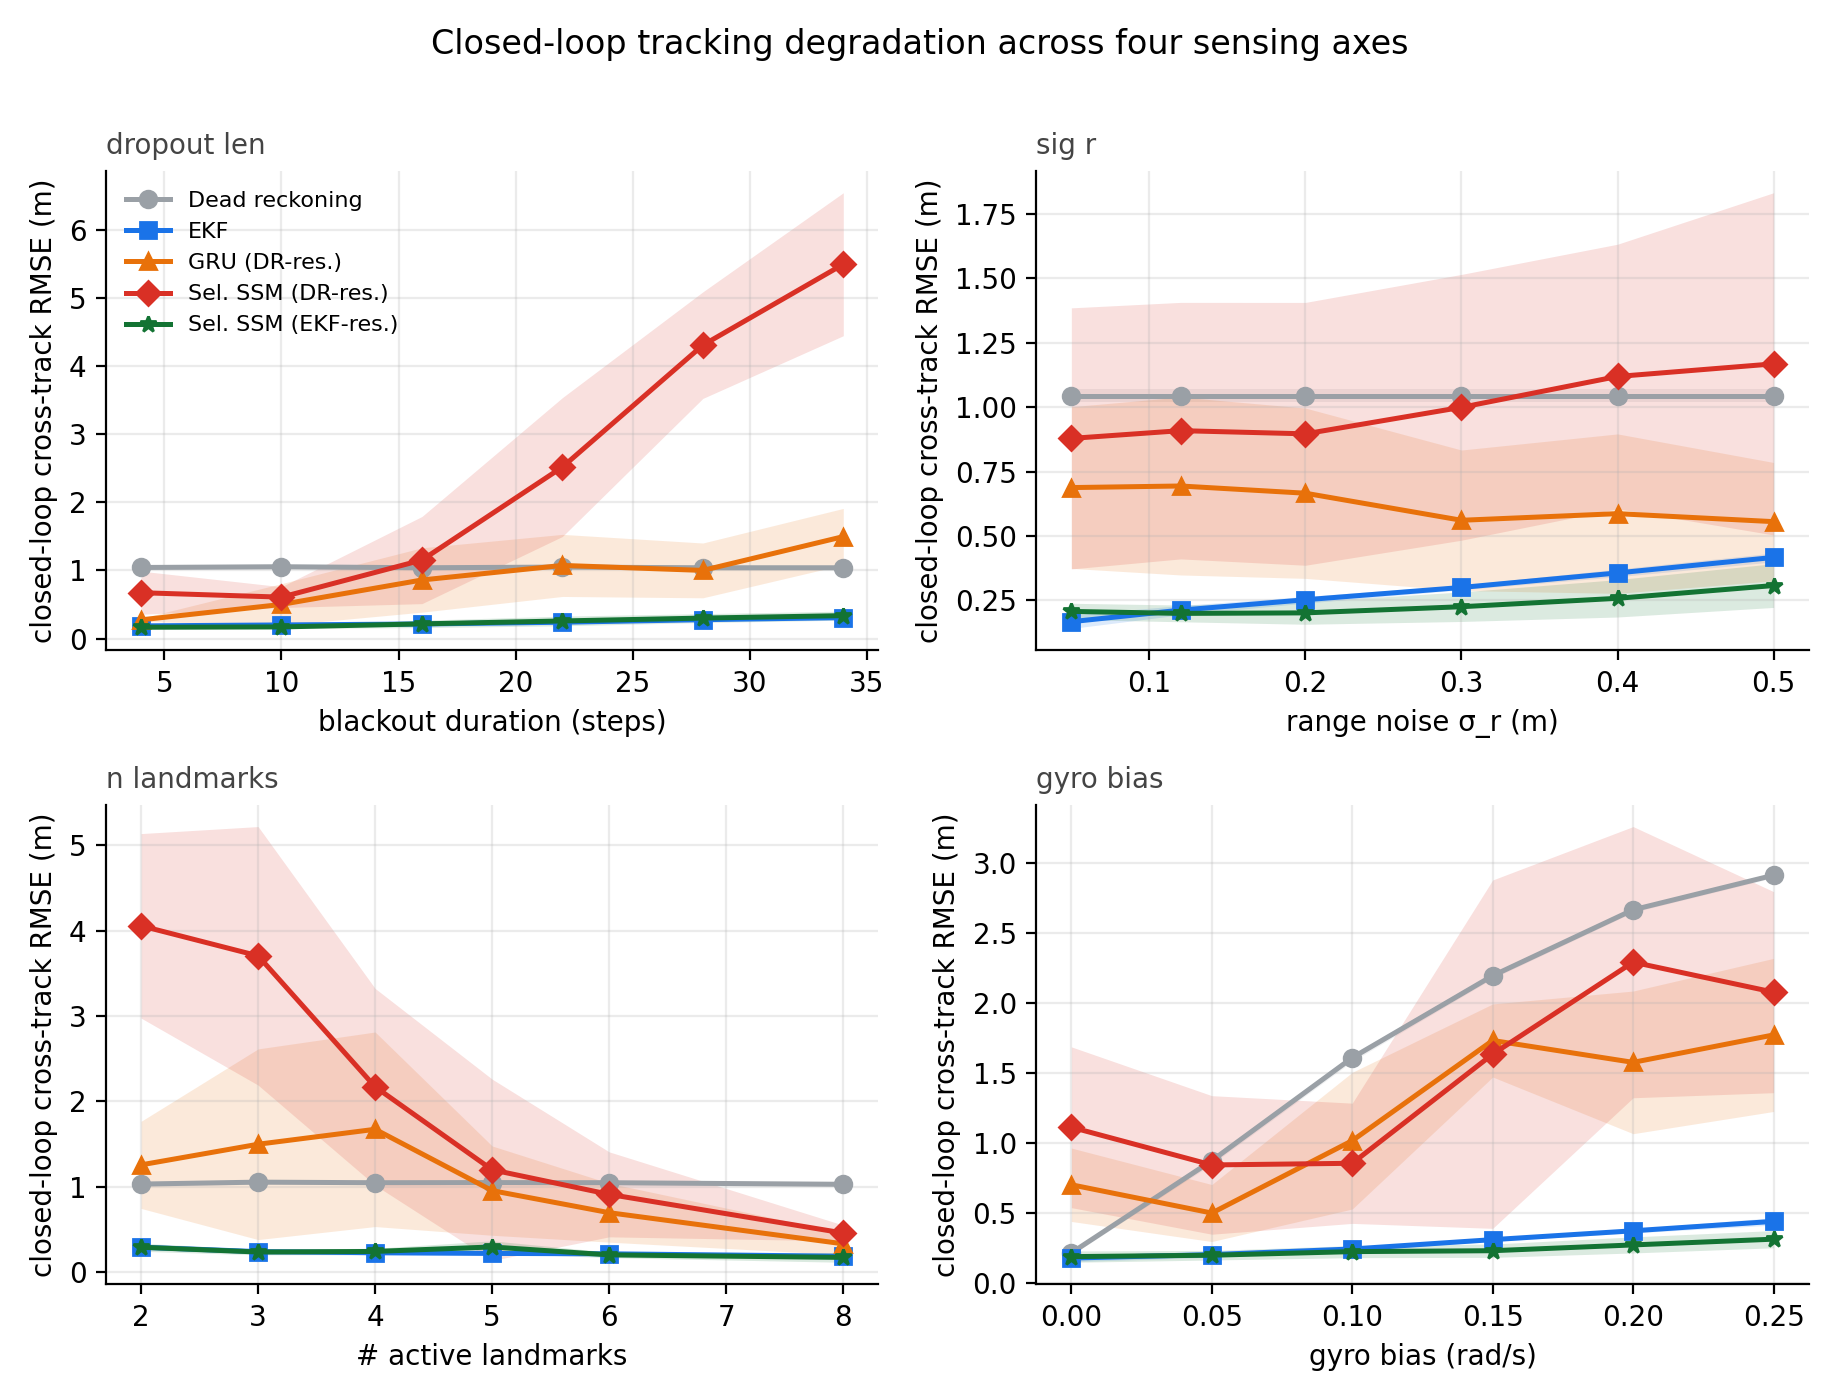
\includegraphics[width=0.92\linewidth]{fig_sweeps.png}
\caption{Closed-loop cross-track RMSE vs.\ each degradation axis (mean $\pm 95\%$ CI over 10 seeds).
Learned EKF-residual observers hug the EKF and pull ahead under heavy measurement noise and
odometry bias, but not under long blackouts or extreme landmark sparsity.}
\label{fig:sweeps}
\end{figure}

\subsection{Objective mismatch: does open-loop RMSE predict control?}
This is the central question. Figure~\ref{fig:mismatch} (left) scatters open-loop position RMSE
against closed-loop cross-track error for every core observer across every swept condition. The
global rank correlation is high (Spearman $\rho=0.89$, $p<10^{-40}$): coarsely, better estimators
do control better, and open-loop RMSE is not useless. But the relationship is loose where it
counts---the Pearson correlation of magnitudes is only $r=0.44$, and per-condition rank agreement
drops as low as $\rho=0.40$. Most importantly (Figure~\ref{fig:mismatch}, right), the
\emph{winner}---the observer with the lowest open-loop RMSE---is not the best closed-loop controller
in $7$ of $24$ conditions ($29\%$). Selecting an observer by open-loop RMSE therefore picks a
suboptimal controller almost a third of the time. Concrete inversions appear even between siblings:
at nominal, \obs{GRU-DR} has lower open-loop RMSE than \obs{SSM-DR} yet worse closed-loop tracking;
and within a single observer, position RMSE and cross-track error themselves diverge (at
$b_g=0.25$ the SSM-EKF ties the EKF on position but improves cross-track by $29\%$).

\begin{figure}[t]
\centering
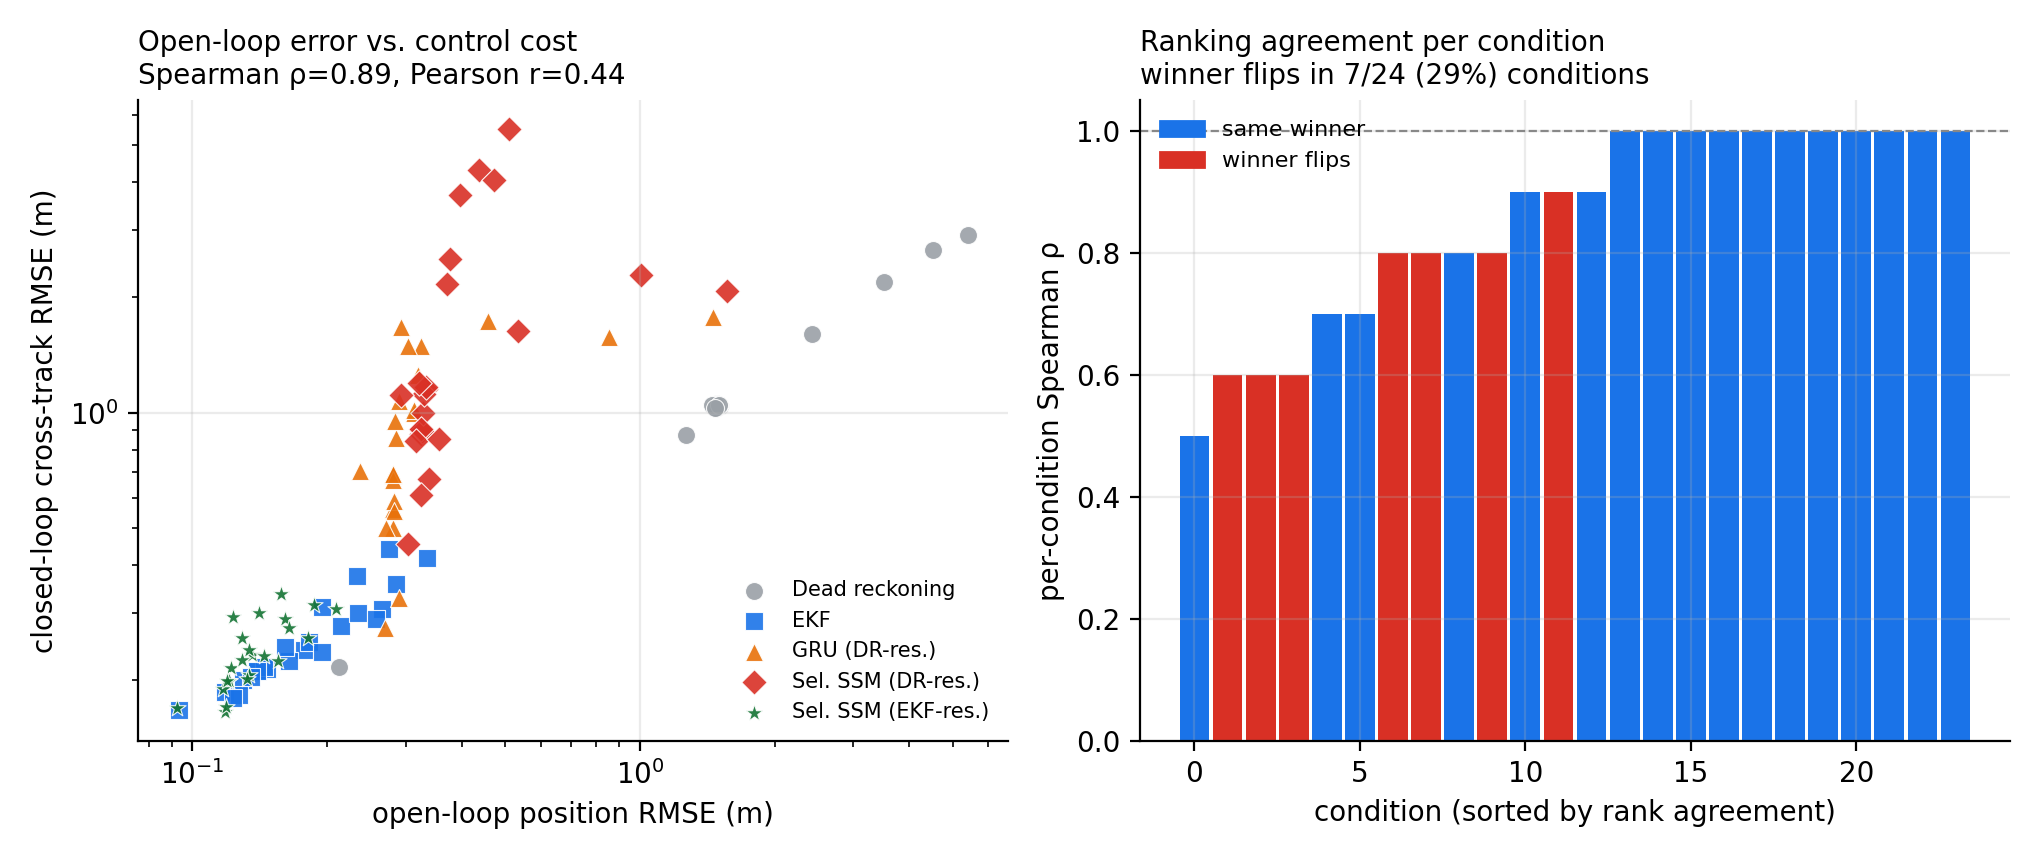
\includegraphics[width=0.98\linewidth]{fig_mismatch.png}
\caption{\textbf{Objective mismatch.} Left: open-loop position RMSE vs.\ closed-loop cross-track
error across all conditions (log--log); the association is directionally right but magnitude-loose
($\rho=0.89$, $r=0.44$). Right: per-condition rank agreement; in red conditions the best open-loop
estimator is \emph{not} the best controller---$29\%$ of all conditions.}
\label{fig:mismatch}
\end{figure}

\subsection{Compound stress: the sharpest inversion}
Table~\ref{tab:compound} pushes all four axes to hard values simultaneously (heavy slip and gyro
bias, high range noise, sparse landmarks, long blackouts). Here the mismatch is starkest: both
learned EKF-residual observers slash \emph{open-loop} position RMSE by $\sim$$43\%$ ($0.83\to0.45$--$0.47$\,m),
yet on \emph{closed-loop} cross-track the selective SSM-EKF is $10\%$ \emph{worse} than the plain
EKF, and the two are statistically indistinguishable within CI. A large, real improvement in
estimation accuracy simply did not transfer to control---objective mismatch in its cleanest form.
(GRU-EKF happens to help here, but the SSM-EKF's failure at its own best estimation regime is the
point.)

\begin{table}[t]
\centering\small
\caption{Compound-stress condition (all axes hard at once), mean over 10 seeds $\pm 95\%$ CI.
Learned EKF-residual observers cut open-loop RMSE sharply while \emph{not} improving closed-loop
cross-track error.}
\label{tab:compound}
\begin{tabular}{lccc}
\toprule
Observer & CL Cross-track (m) & CL Pos (m) & Open-loop Pos (m) \\
\midrule
Dead reckoning        & $2.528\pm.01$ & $4.818\pm.03$ & $3.289\pm.38$ \\
EKF                   & $1.324\pm.09$ & $1.467\pm.36$ & $0.829\pm.07$ \\
GRU (EKF-residual)    & $\mathbf{1.052\pm.33}$ & $1.222\pm.42$ & $0.447\pm.05$ \\
Sel.\ SSM (EKF-res.)  & $1.459\pm.16$ & $1.496\pm.35$ & $\mathbf{0.472\pm.04}$ \\
Sel.\ SSM (DR-res.)   & $4.228\pm1.36$ & $5.734\pm1.42$ & $0.798\pm.10$ \\
\bottomrule
\end{tabular}
\end{table}

\subsection{What makes a learned observer closed-loop-stable?}
Two ablations (Table~\ref{tab:nominal}, Figure~\ref{fig:ablation}) isolate the ingredients. Removing
\emph{selectivity} from the SSM or removing \emph{mask awareness} barely changes open-loop RMSE
($0.30$--$0.59$\,m, still far better than dead reckoning) but is catastrophic closed-loop
(cross-track $2.3$--$3.3$\,m, divergence up to $0.58$). The observer cannot tell present from absent
measurements and its corrections destabilize the loop. Separately, the \emph{anchor} matters: every
dead-reckoning-residual learned observer is open-loop-competitive but closed-loop-poor, whereas the
same cells on an EKF anchor are stable. The physics prior does the heavy lifting; the learned part
is a correction that is only safe when the base is sound and the gating respects measurement
availability.

\begin{figure}[t]
\centering
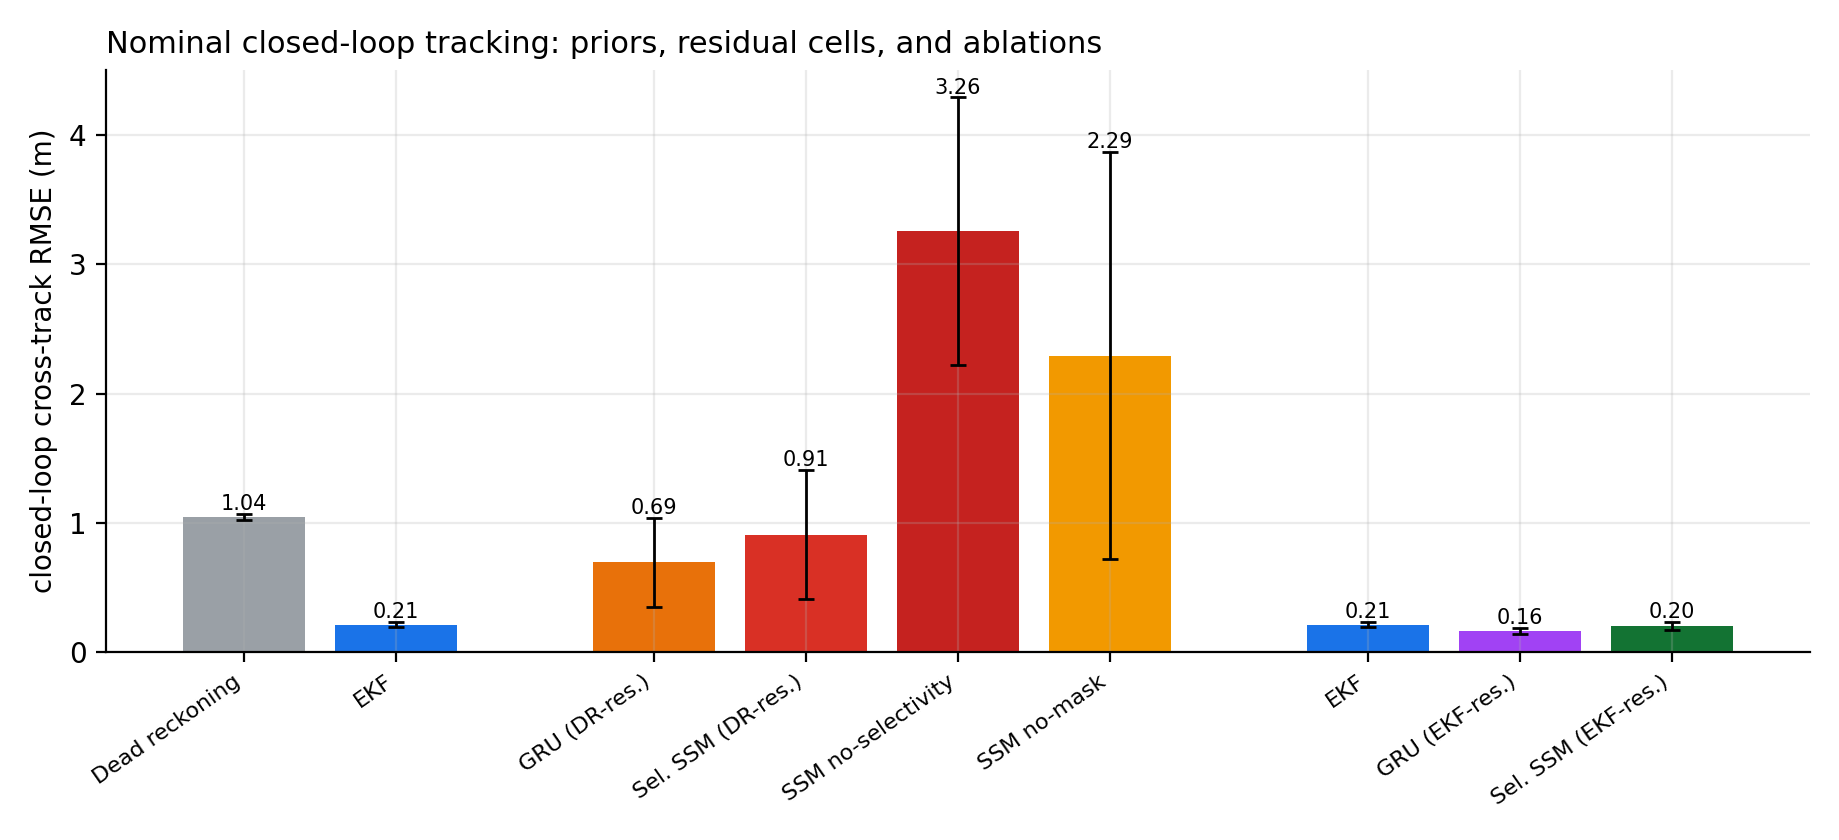
\includegraphics[width=0.9\linewidth]{fig_ablation.png}
\caption{Nominal closed-loop cross-track RMSE by group. The EKF anchor yields stable low-error
control; dead-reckoning-residual observers are worse and higher-variance; removing selectivity or
mask-awareness is catastrophic despite competitive open-loop RMSE (Table~\ref{tab:nominal}).}
\label{fig:ablation}
\end{figure}

\subsection{Recovery through blackouts}
Figure~\ref{fig:ts} shows position error over a single run with periodic blackouts. Dead reckoning
ratchets upward through each gap and never recovers; the EKF and the selective SSM-EKF stay bounded,
snapping back when measurements return. This is the mechanism behind the sweep and mismatch
results: the controller inherits whatever error the estimator accumulates during a gap.

\begin{figure}[t]
\centering
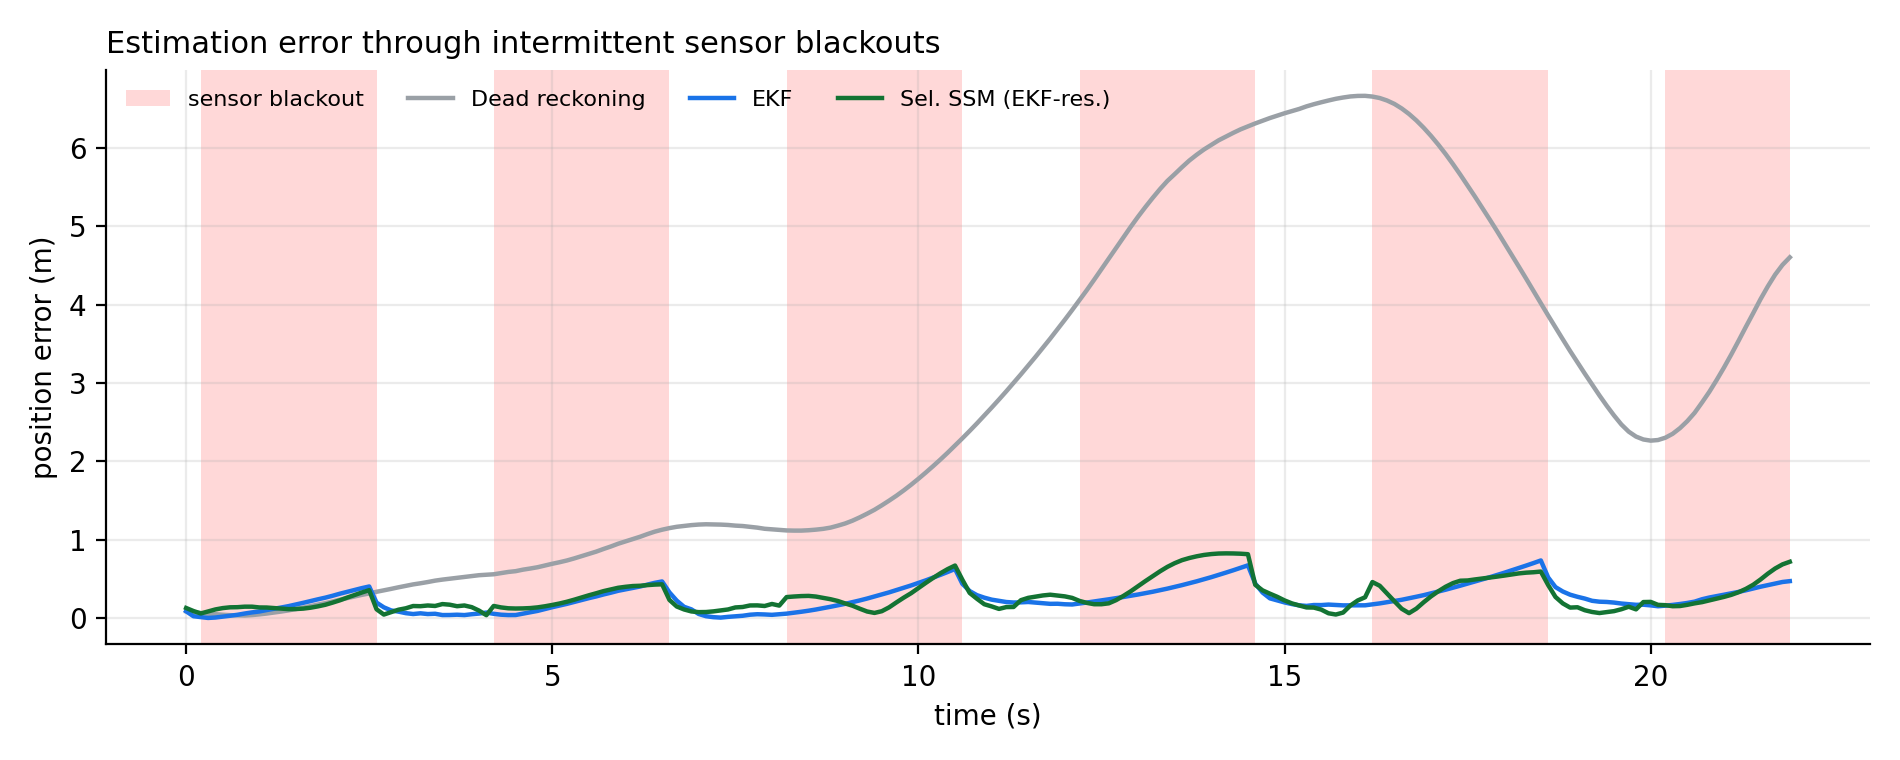
\includegraphics[width=0.92\linewidth]{fig_timeseries.png}
\caption{Position error through intermittent blackouts (shaded). Dead reckoning drifts without
bound; model-based and physics-anchored learned observers stay bounded and recover on measurement
return.}
\label{fig:ts}
\end{figure}

\section{Discussion}
\textbf{Open-loop RMSE is a biased proxy.} It is not worthless---rankings agree on average---but it
is unreliable exactly at the decision that matters, choosing the best observer, and it can reward
estimators that are unstable in the loop. The failure is not random noise: it is structural, because
open-loop replay never exposes the estimator to the state distribution its own control errors
induce. An observer optimized and judged off-loop is judged off-distribution.

\textbf{The physics prior is load-bearing.} The dead-reckoning-residual observers show that a model
can be an excellent open-loop estimator and a poor controller; anchoring the residual on an EKF
makes the same learned cell closed-loop-stable. This favors hybrid designs that keep an analytic
recursion and learn only a correction, echoing KalmanNet~\cite{kalmannet} but evaluated in the loop.

\textbf{Selectivity is about knowing when you are blind.} Mask-aware, selective gating is what lets
a learned observer stop trusting phantom measurements during blackouts. Its absence is invisible to
open-loop RMSE but fatal closed-loop---a second reason off-loop metrics mislead.

\textbf{Limitations.} The study is simulation-only with a known landmark map, one controller family
(pure pursuit, with Kanayama available), single-seed training, and a compact SSM rather than a
full Mamba block; unknown-map SLAM, multi-seed training, and hardware are natural next steps. The
positive closed-loop wins for the hybrids are regime-specific (noise and bias), not universal, and
we report them as such.

\section{Conclusion}
Estimators are chosen by open-loop accuracy but used in closed loops. Across a controlled study of
classical and selective-state-space learned observers under intermittent sensing, open-loop RMSE
predicted closed-loop tracking only directionally: it selected the wrong observer in $29\%$ of
conditions, and our best-estimating learned model failed to improve control under compound stress.
Physics-anchored, mask-aware selective residuals were the only learned observers that were reliably
stable in the loop, and helped most where measurements were frequent but mis-modeled. The practical
takeaway is simple and, we think, under-practiced: evaluate learned filters in the loop.

\begin{thebibliography}{99}
\small
\bibitem{thrun} S.\ Thrun, W.\ Burgard, and D.\ Fox, \emph{Probabilistic Robotics}. MIT Press, 2005.
\bibitem{siegwart} R.\ Siegwart, I.\ R.\ Nourbakhsh, and D.\ Scaramuzza, \emph{Introduction to Autonomous Mobile Robots}, 2nd ed. MIT Press, 2011.
\bibitem{kanayama} Y.\ Kanayama et al., ``A stable tracking control method for an autonomous mobile robot,'' in \emph{Proc.\ IEEE ICRA}, 1990, pp.\ 384--389.
\bibitem{coulter} R.\ C.\ Coulter, ``Implementation of the pure pursuit path tracking algorithm,'' CMU Robotics Inst., Tech.\ Rep.\ CMU-RI-TR-92-01, 1992.
\bibitem{dvbf} M.\ Karl et al., ``Deep variational Bayes filters,'' in \emph{Proc.\ ICLR}, 2017.
\bibitem{rkn} P.\ Becker et al., ``Recurrent Kalman networks,'' in \emph{Proc.\ ICML}, 2019, pp.\ 544--552.
\bibitem{dpf} R.\ Jonschkowski, D.\ Rastogi, and O.\ Brock, ``Differentiable particle filters,'' in \emph{Proc.\ RSS}, 2018.
\bibitem{kalmannet} G.\ Revach et al., ``KalmanNet: Neural network aided Kalman filtering for partially known dynamics,'' \emph{IEEE Trans.\ Signal Process.}, vol.\ 70, pp.\ 1532--1547, 2022.
\bibitem{latentode} Y.\ Rubanova, R.\ T.\ Q.\ Chen, and D.\ Duvenaud, ``Latent ODEs for irregularly-sampled time series,'' in \emph{NeurIPS}, vol.\ 32, 2019.
\bibitem{s4} A.\ Gu, K.\ Goel, and C.\ R\'e, ``Efficiently modeling long sequences with structured state spaces,'' in \emph{Proc.\ ICLR}, 2022.
\bibitem{mamba} A.\ Gu and T.\ Dao, ``Mamba: Linear-time sequence modeling with selective state spaces,'' in \emph{Proc.\ COLM}, 2024.
\bibitem{lambert} N.\ Lambert, B.\ Amos, O.\ Yadan, and R.\ Calandra, ``Objective mismatch in model-based reinforcement learning,'' in \emph{Proc.\ L4DC}, 2020, pp.\ 761--770.
\end{thebibliography}

\end{document}
